\documentclass{article}
\usepackage[spanish]{babel}
\usepackage[pdftex]{graphicx,color} 
\usepackage[utf8]{inputenc}
\usepackage{listings}
\usepackage{colortbl}
\usepackage{textcomp}
\usepackage{listings}
\usepackage{color}
\usepackage{wrapfig}
\usepackage{amsfonts}
\usepackage{amssymb}
\usepackage{algorithmic}
\usepackage{algorithm}
\usepackage[export]{adjustbox}
%\usepackage{amslatex}
\definecolor{lbcolor}{rgb}{0.9,0.9,0.9}
\lstset{
        backgroundcolor=, %\color{lbcolor},
        tabsize=4,
        rulecolor=,
        language=C,
        basicstyle=\scriptsize,
        upquote=true,
        aboveskip={1.5\baselineskip},
        %columns=fixed,
        showstringspaces=false,
        extendedchars=true,
        breaklines=true,
        prebreak = \raisebox{0ex}[0ex][0ex]{\ensuremath{\hookleftarrow}},
        frame=single,
        showtabs=false,
        showspaces=false,
        showstringspaces=false,
        identifierstyle=\ttfamily,
        keywordstyle=\color[rgb]{0,0,1},
        commentstyle=\color[rgb]{0.133,0.545,0.133},
        stringstyle=\color[rgb]{0.627,0.126,0.941},
	literate={á}{{\'a}}1
	{ã}{{\~a}}1
	{é}{{\'e}}1
	{ó}{{\'o}}1
	{í}{{\'i}}1
	{ñ}{{\~n}}1
	{¡}{{!`}}1
	{¿}{{?`}}1
	{ú}{{\'u}}1
	{Í}{{\'I}}1
	{Ó}{{\'O}}1
}

\topmargin -0.5in
\textwidth 6.8in
\textheight 9.0in
\oddsidemargin 0.0in
\evensidemargin 0.0in

\usepackage{enumitem}
\usepackage{multirow}
\usepackage{hhline}
\usepackage{multicol}
%ointpoints{punto}{puntos}

\begin{document}
\vspace{.5pc}
\centerline{\sc Clase Activa 3}
\centerline{\sc ELO320 - Estructura de Datos y Algoritmos}
\centerline{\sc Prof. Nicolás Gálvez Ramírez}
\vspace{2pc}
%\noindent {\bf Instrucciones}:
%\begin{itemize}
%    \item Conteste cada pregunta en una hoja separada. Éstas serán entregadas de tal forma al finalizar el certamen.
%    \item Si decide no contestar una pregunta, debe entregar una hoja sin respuestas en su lugar. 
%    \item Rotule claramente cada una de sus hojas con su Nombre Completo, Rol USM y Número de Paralelo.
%    \item El certamen tiene una duración de 60 minutos.
%\end{itemize}

%\noindent {\bf Preguntas}
%\medskip
\begin{itemize}

\begin{minipage}[h]{0.45\textwidth}
\item \textbf{Arreglo}: Conjunto homogéneo y ordenado de un tipo de datos. Se identifican por su posición relativa mediante un \emph{índice} encerrado con paréntesis cuadrado ([], parte de índice 0).

\begin{lstlisting}[language=C, basicstyle=\scriptsize, escapeinside={|}{|}]
int main(){
	
	int arr[6]; // 6 enteros creados en arr
	arr[3] = 222; // Al cuarto elemento de arr se le asigna 222
}
\end{lstlisting}
\begin{center}
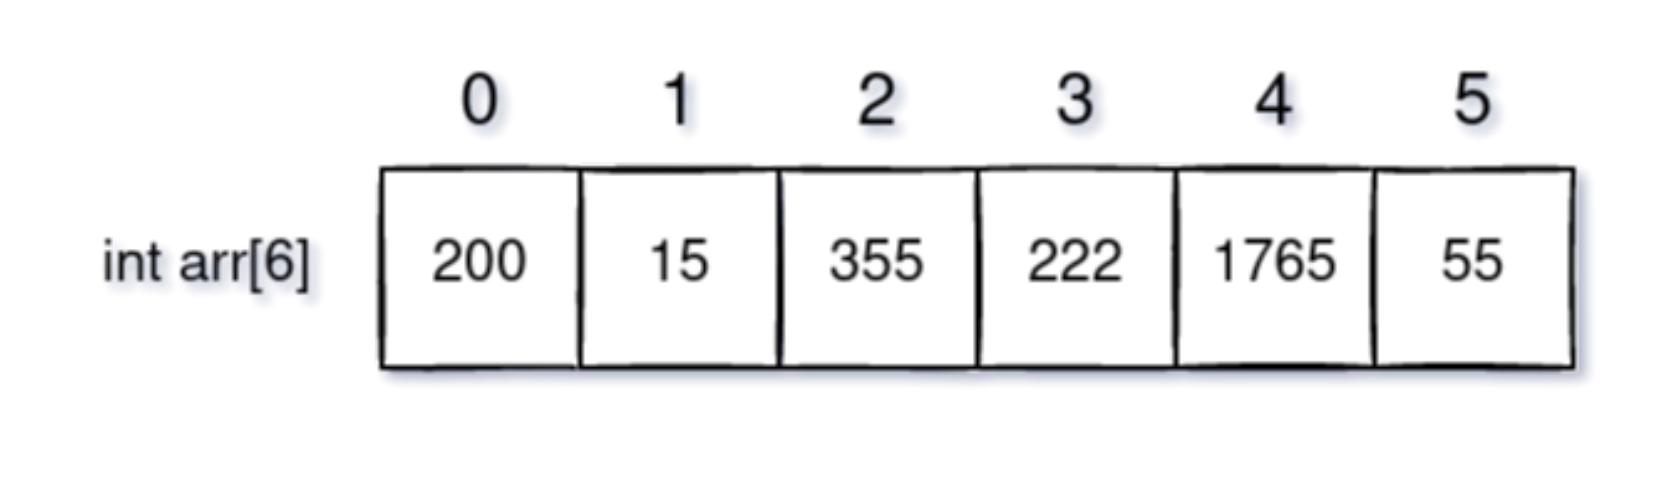
\includegraphics[width=.9\linewidth]{images/array.png}
\end{center}
\end{minipage}
\hspace{0.5cm}
\begin{minipage}[h]{0.45\textwidth}
\item \textbf{String}: Estructura de datos para representar palabras. Usa arreglos de \texttt{char} y el caracter especial '\textbackslash0'.
\begin{lstlisting}[language=C, basicstyle=\scriptsize, escapeinside={|}{|}]
// Los string terminan con '\0' (fin de string) 
// '\0' ocupa 1 char en el string
char str[6] = "hola"; //String de largo máximo 5. 
str[3] = 'i'; // ¿Qué hace? 
printf("|\%|s\n", str);
\end{lstlisting}
\begin{center}
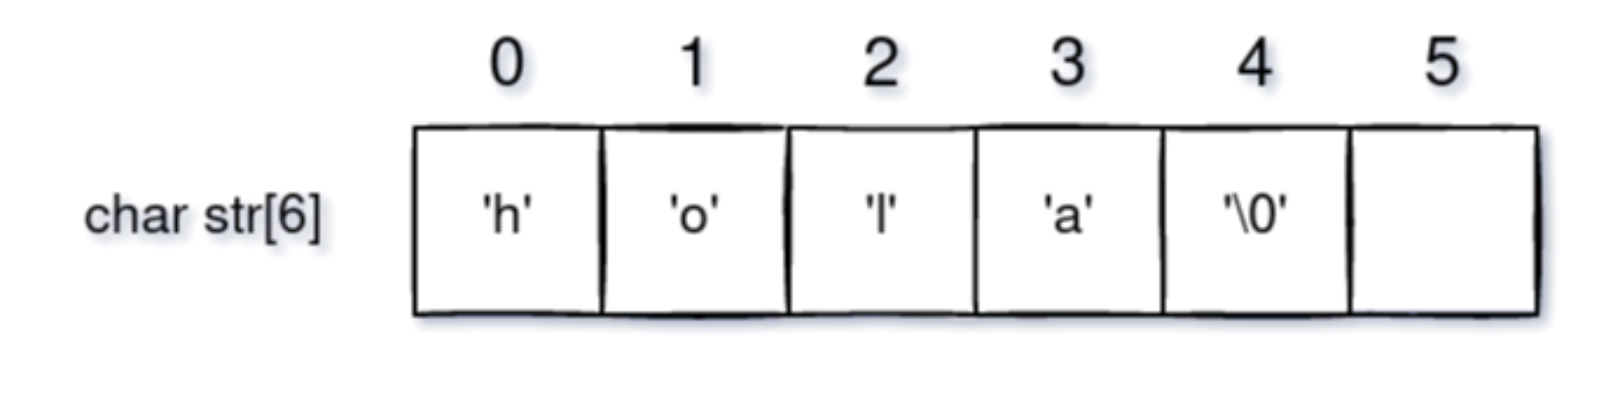
\includegraphics[width=.9\linewidth]{images/string.png}
\end{center}

\end{minipage}

\begin{minipage}[h]{0.45\textwidth}
\item \textbf{Arreglo multidimensional}: Conjunto de datos en varias dimensiones. Arreglo con variados [].
\begin{lstlisting}[language=C, basicstyle=\scriptsize, escapeinside={|}{|}]
#include<stdio.h>

int main(){
	char nom[10] = "Camilo";
	char a[5][20] = {"Juan", "Francisco", "Pedro"};	
	int b[3][3] = {{1,2,3}, {4,5,6}, {7,8,9}}, i, j;

	for(i=0;i<3;i++){
		for(j=0;j<3;j++) //¿Qué pasó con las llaves? 
			printf("|\%|d ", b[i][j]);
		printf("\n");
	}
}
\end{lstlisting}

Nótese que los arreglos pueden ser \textbf{inicializados}, pero \textbf{no asignados}.
\end{minipage}
\hspace{0.5cm}
\begin{minipage}[h]{0.45\textwidth}
\item \textbf{Recorrer Arreglo}: Con cualquier ciclo se puede hacer, pero \textbf{for} es lo más cómodo. 
\begin{lstlisting}[language=C, basicstyle=\scriptsize, escapeinside={|}{|}]
#include<stdio.h>

int main(){
	int i;
	float a[5];
	
	for(i=0;i<5;i++){
		float val; //¿Cuántas veces nace y muere val?
		scanf("|\%|f", &val);
		a[i]=val;
	} //¿Cómo reducir este código?

}
\end{lstlisting}
\end{minipage}

\end{itemize}
\end{document}

